\documentclass[Dissertation.tex]{subfiles}

\begin{document}


\begin{center}
\textbf{\section{Introduction}}
\end{center}

\subsection{Description}
Students who suffer from personal problems usually fill out the \textit{Extenuating Circumstances Form (ECF)} which then allows the examination board (the scrutiny committee) to consider their problems. The process usually begins with the student submitting the form and being reviewed if the circumstance is true and if there is enough evidence to support this. In situations where there is not enough evidence, the committee asks the student to provide more evidence and then processes the form accordingly, for example the committee may ask the student to present a death certificate. The form at this point has detailed information about the personal problem but from here on, only the general problem (without including details of the specific problem the student is facing) is taken ahead to the other departments and also added to the Students Record to allow leniency in terms of examinations and other assignments. Information regarding the ECFs can be found on the University Of Sheffield's page.\cite{ecfuni}

\subsection{Project}
The main aim of this project would be to build a system which can achieve confidentiality, ease of access and at the same time reduce the paperwork required. Data will be stored on an encrypted and secure database allowing only authorised departments to access the only information needed.

\begin{center}
\textbf{\section{Analysis}}
\end{center}

\subsection{Problem}
Once the forms have been filled there may be a request for more evidence or the forms may need to be duplicated with less details to other departments and also fed into the system to be accessed under the Student Report. This reduces confidentiality and a lot of confusion. Instances where a student submits multiple ECFs or after recovery re-submit another form disorients the gathering of these forms and leads to mistakes being made. Forms are sometimes required for an appeal and multiple/lost forms produces a biased outcome. 

\subsection{Possible Techniques}
There are two possibilities to achieving a secure and improved system. The first being a web-based system and the second being a mobile phone application. 

Django, a Python based web developing system would be a great tool for solving the problems. It is built to be one of the most secure language compared to other languages such as .Net, ASP, Java, PHP or Ruby\cite{djangovslaravel}\cite{securelanguage}. A web based system would ensure that everybody can access the system and find previous records without having to re-submit a new form and at the same time with Django’s security the forms shall remain secure and confidential. With Python allowing and sharing data between the already existing system will also be possible. 

Alternatively a mobile phone application would allow students to submit their problems directly from their phone and then these can be accessed by the committee using the same application and process the forms accordingly. 

\begin{center}
\textbf{\section{Plan Of Action}}
\end{center}

\subsection{Gantt Chart}
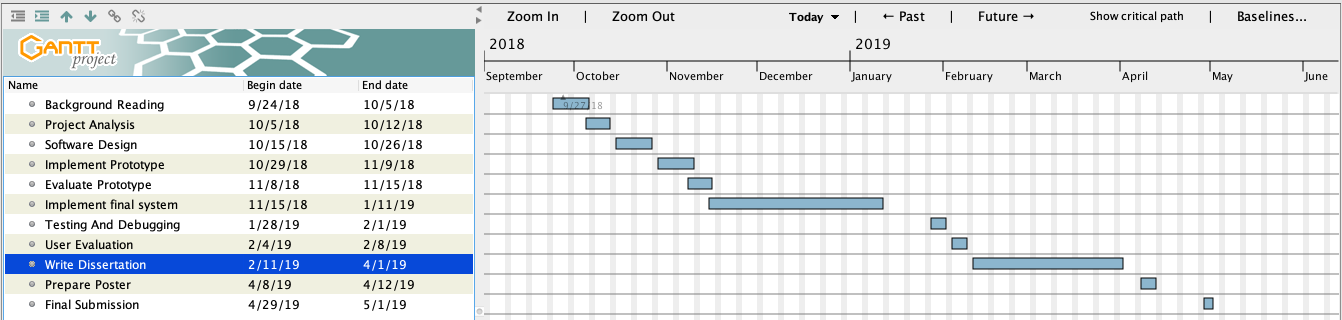
\includegraphics[scale=0.57]{images/Gantt.png} 

\subsection{Plan}
As shown on the Gantt chart above, the background research and reading has already started and I soon plan to start collecting as much information as i can based on the two possible techniques mentioned above. After the research has been successfully completed and i have finalised the main technique i shall start coding the system. By the end of this semester I should have completed at least 50\% of the coding and by mid January the final system should be up and running. Every system requires Testing and Debugging which will continue from mid Jan till the beginning of February. I’ll have approximately two and a half months then to start and complete my dissertation by the beginning of April. Lastly I’ll use the first week of April to complete the poster required and make any last changes required. 

\end{document}
